\chapter{Domain Driven Design}
\section{Ubiquitous Language}
\begin{description}
	\item[Klasse] Die Klasse des Charackters. Sie bestimmt Lebenspunkte, Sprachen, Heilungsmöglichkeiten uvm. Sie hat einen direkten Einfluss auf die Spielweise des Charackters. Sie gehört zur Ubiquitous Language, dar sie einen spezielle Eigenschaft des Charackters beschreibt. Andere könnten unter diesem Begriff vor allem im Programmier Umfeld unterschiedliche Dinge
	\item[Rasse] Die Rasse des Charackters. Sie bestimmt Attribut Boni, die Geschwindigkeit, Sprachen, Alter und Größe. Somit hat sie einen gr0ßen Einfluss auf die äußerliche Erscheinung des Charackters. Sie ist Teil der Ubiquitous Language, da sie im Domänen Umfeld Einfluss auf viele Dinge hat. Außenstehende würden diesen Begriff sicherlich meist mit negativen Ausdrücken assoziieren oder ihn allein auf die Hautfarbe eines Menschen beschränken.
	\item[Equipment] Die Ausrüstung die ein Charakter mitführt. Dieser Begriff ist Teil der Ubiquitous language, da es für alle Projekt teilnehmer wichtig ist, was ein Charackter mitführen kann. Dies hat unweigerliche Auswirkungen auf Statuswerte, attackier möglichkeiten uvm.
	\item[HitDice] Die Würfel die ein Spieler würfeln kann, um die Lebenspunkte seines Charakters wieder aufzufüllen. Sie sind Teil der Ubiquitous language, da außenstehende diesen Begriff warscheinlich gar nicht kennen.
\end{description}

\FloatBarrier
\section{Entities}
\begin{figure}[H]
	\centering
	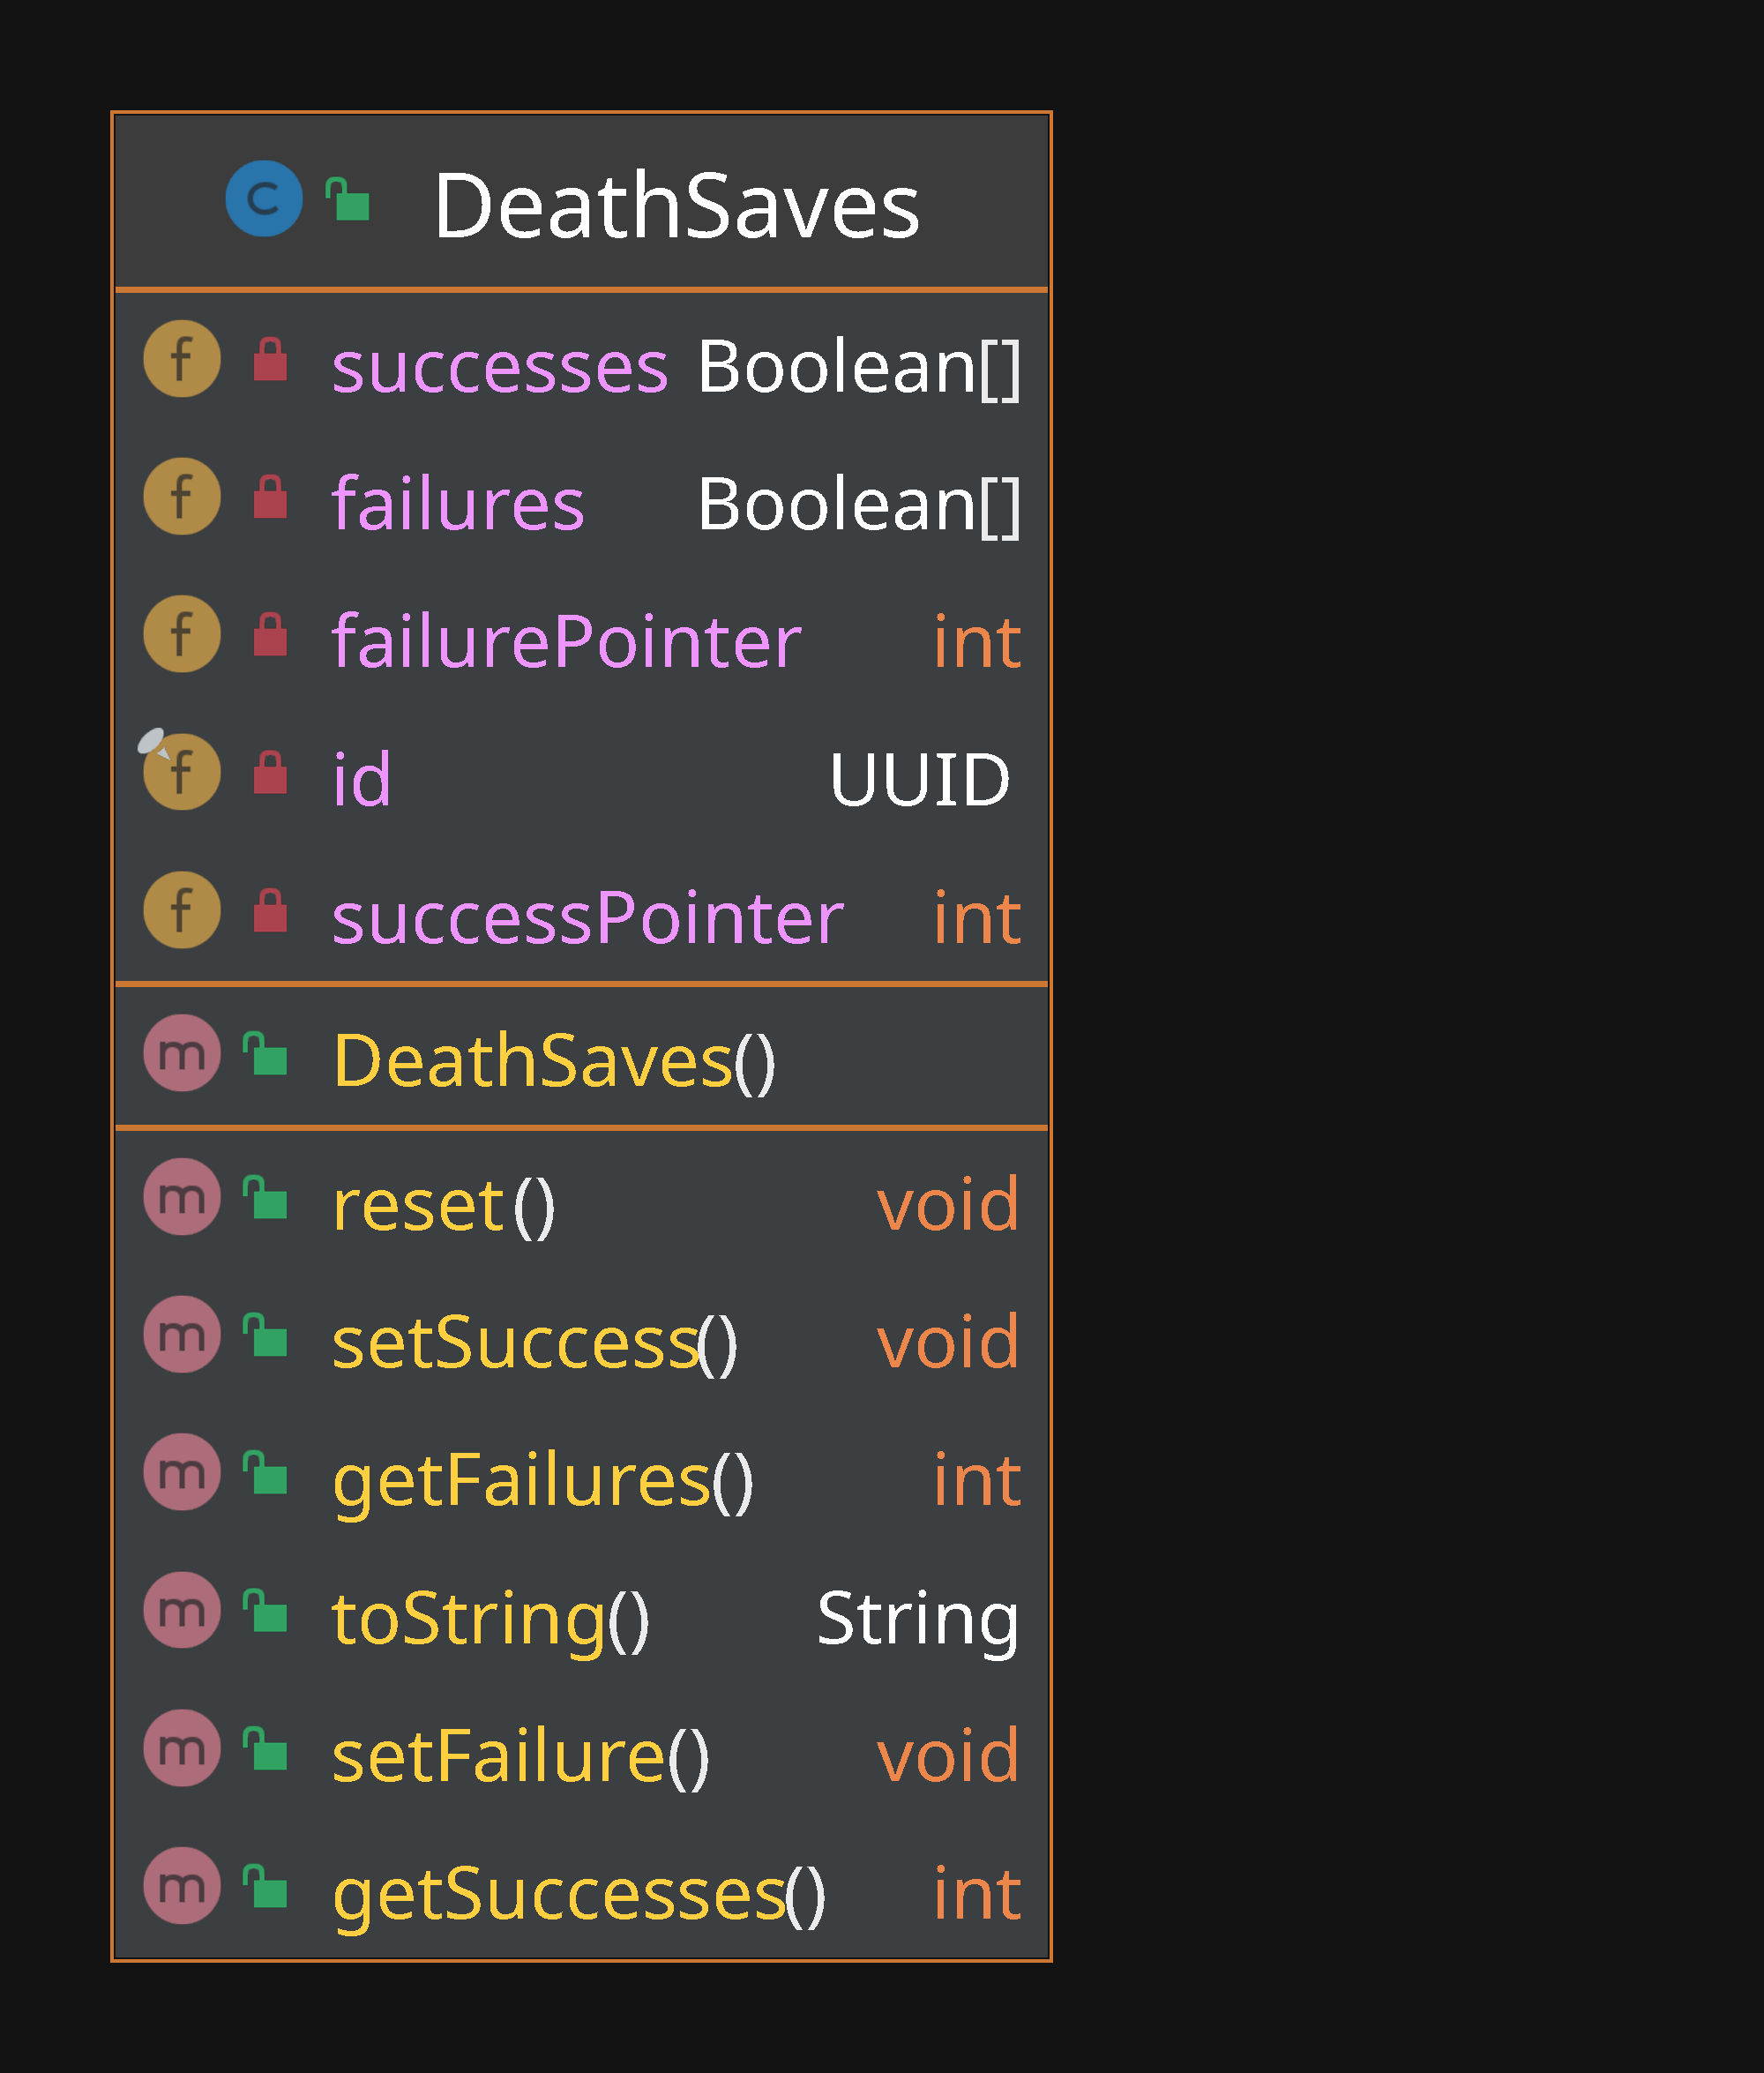
\includegraphics[width=0.4\textwidth]{Bilder/DeathSaves.pdf}
	\caption{UML der DeathSaves Klasse}
	\label{fig:DeathSaves}
\end{figure}
Abbildung \ref{fig:DeathSaves} zeigt eine Entity der Domain Modellierung des DnDCharacterManagers. Die Klasse \texttt{DeathSaves} modelliert die Death Saves eines Spielers. Diese kommen zum Einsatz, falls ein Charackter 0 Lebenspunkte hat. Ist dieser erneut am Zug, wird ein Death Save mit einem D20 geworfen. Dieser kann entweder erfolgreich sein oder fehlschlagen. Hat man 3 erfolgreiche Death Saves kommt man mit 1 Lebenspunkt zurück und kann weiter spielen. Hat man 3 Fehlschläge stirbt der Charackter und kommt auf den Friedhof. Diese Klasse stellt eine Entity dar, da sich ihr Inhalt mit dem Laufe der Zeit verändert. So können Successes oder Failures hinzugefügt werden. Nichts desto trotz muss die Instanz der Klasse eindeutig identifizierbar sein und ist Teil der Charackters, unabhängig ihres Inhalts / der Werte ihrer Attribute. Somit stellt sie eindeutig eine Entity dar und wird mittels einer ID eindeutig identifiziert.

\section{Value Objects}
\begin{figure}[H]
	\centering
	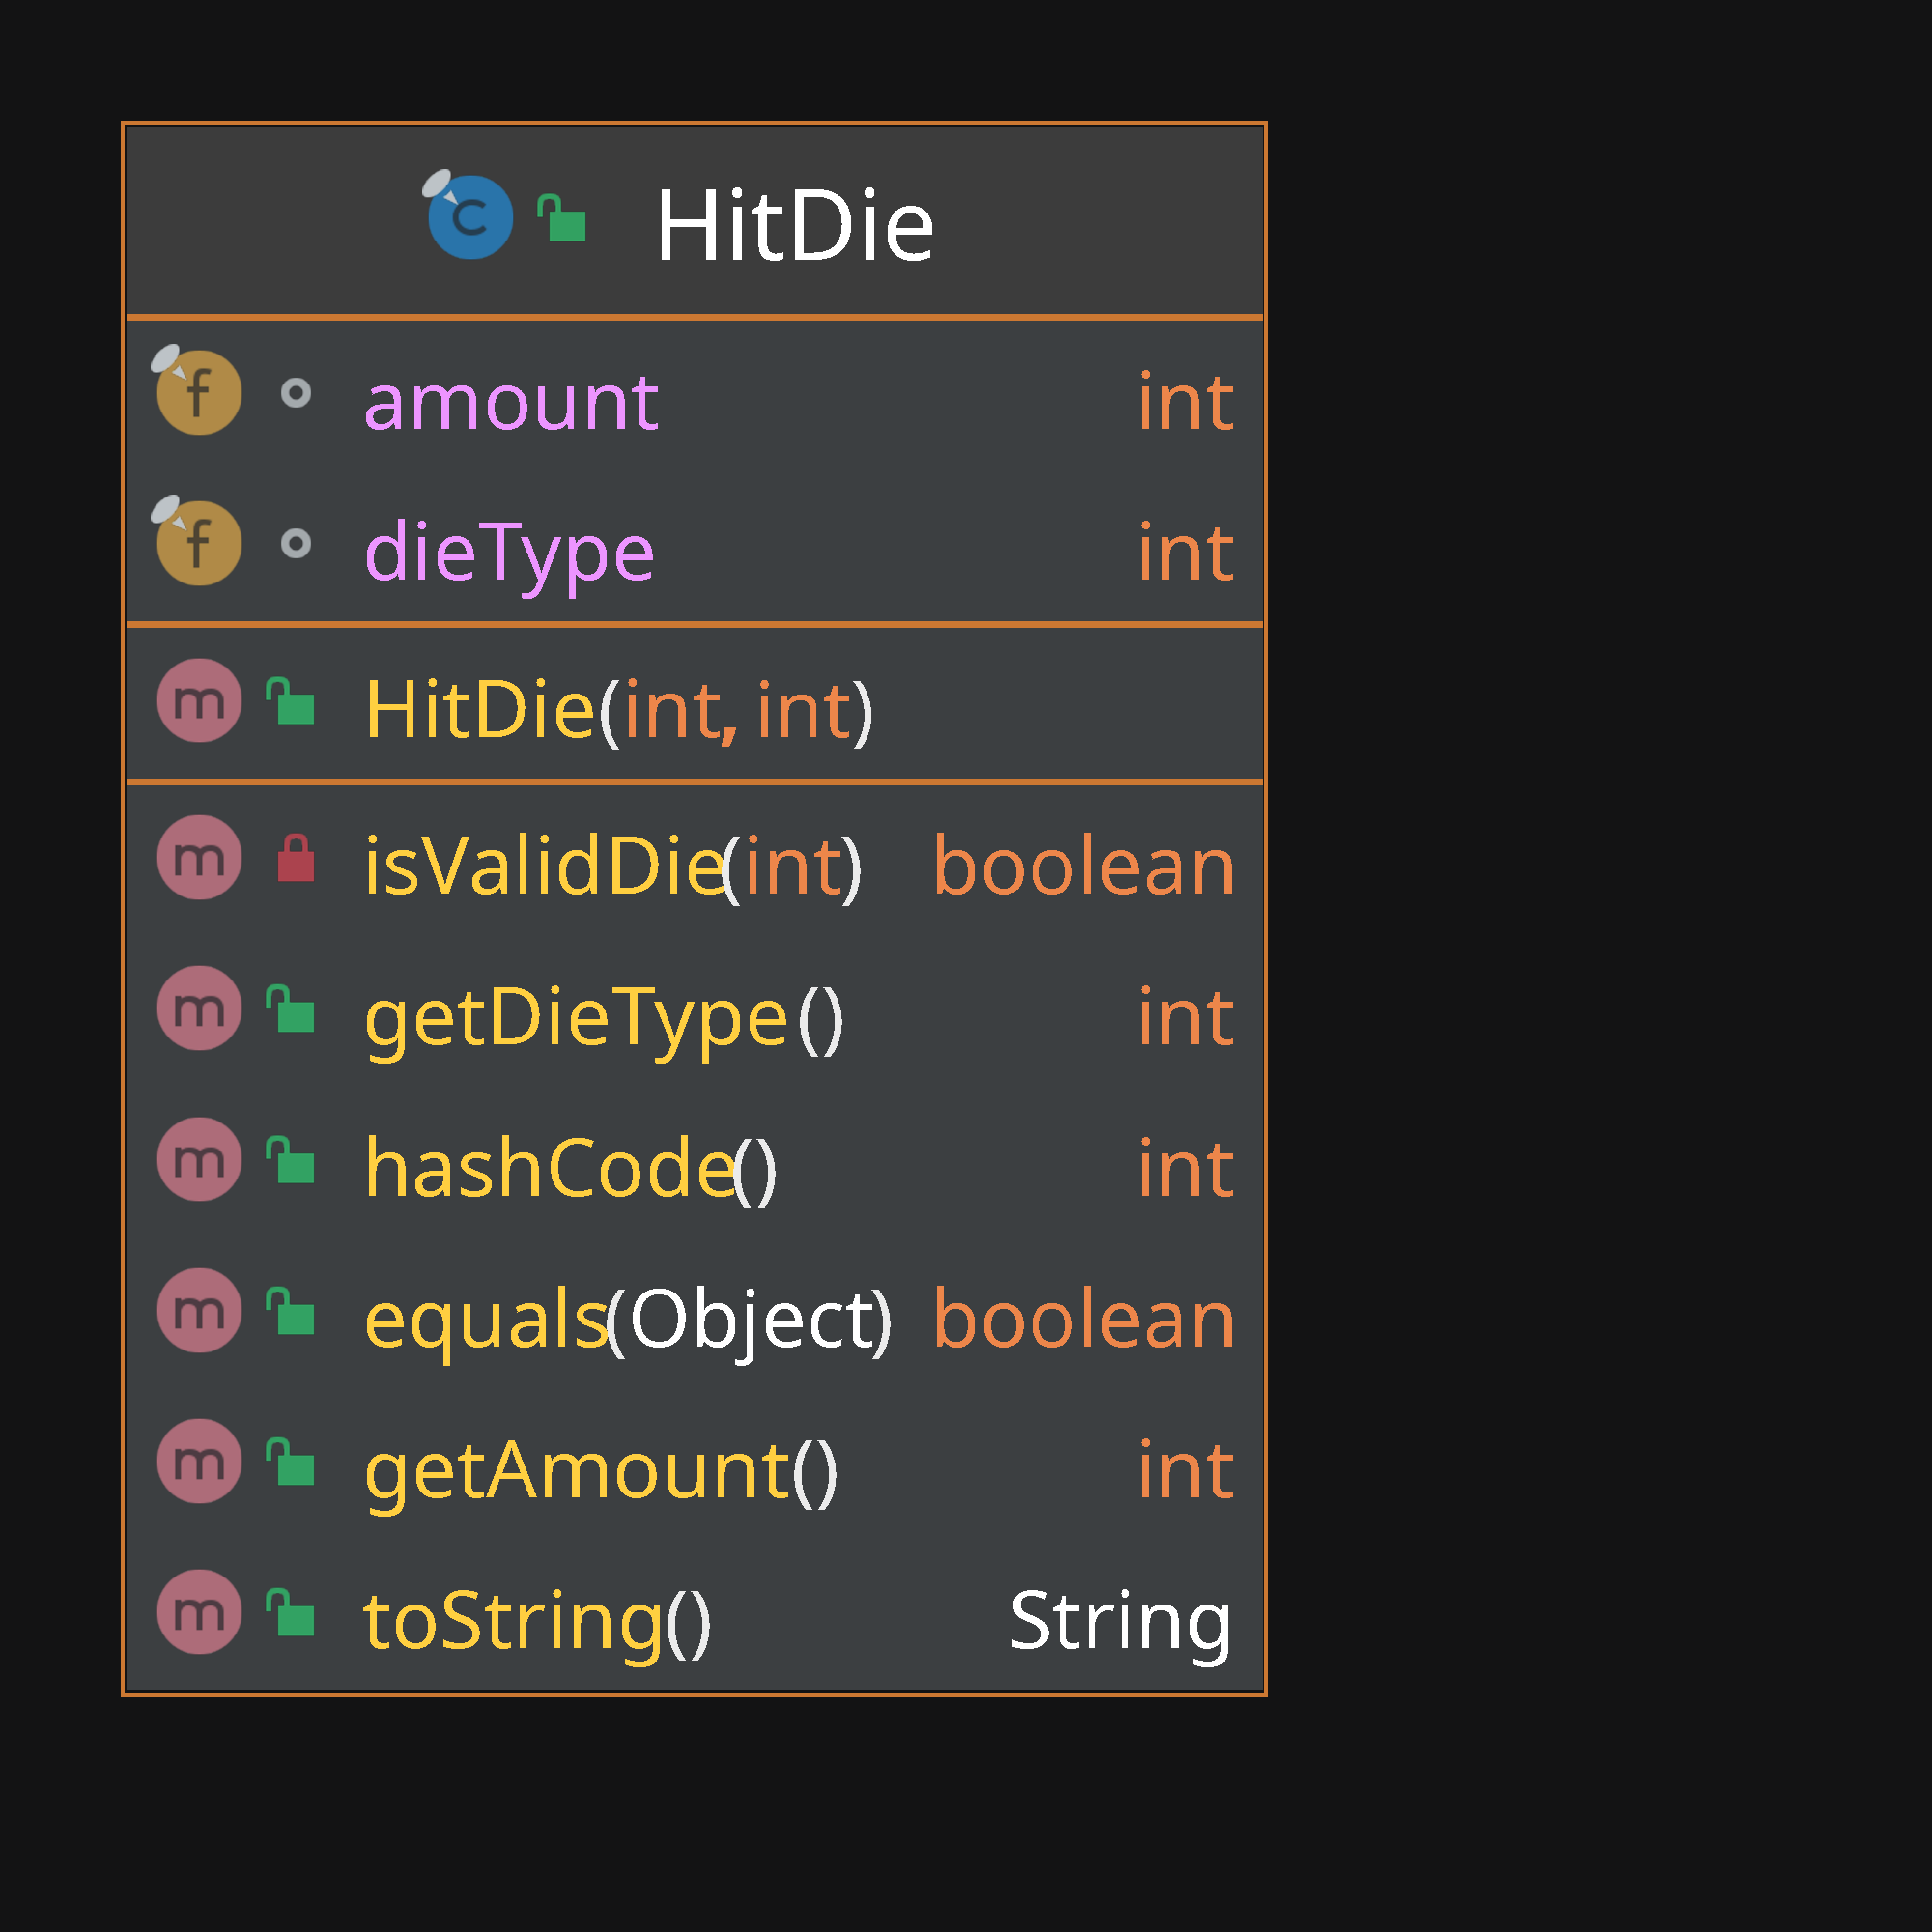
\includegraphics[width=0.4\textwidth]{Bilder/HitDie.pdf}
	\caption{UML der HitDie Klasse}
	\label{fig:HitDie}
\end{figure}
Abbildung \ref{fig:HitDie} zeigt das UML Diagramm der Klasse \texttt{HitDie}. Diese Klasse modelliert einen Würfel für den Angriff, zum heilen oder für verschiedene Checks. Sie stellt also sicher, das ausschließlich die in DnD 5e erlaubten Würfel verwendet werden. Da ein Würfel ausschließlich über seine Merkmale wie die Seitenanzahl, oder wie viele Würfel man zur Verfügung hat identifieziert wird, stellt diese klasse ein Value Object dar. Somit müssen die Attribute \texttt{amount} und \texttt{dieType} auf den selben Hashwert abbilden, damit eine Instanz der Klasse als äquivalent gilt.

\section{Repositories}
\begin{figure}[H]
	\centering
	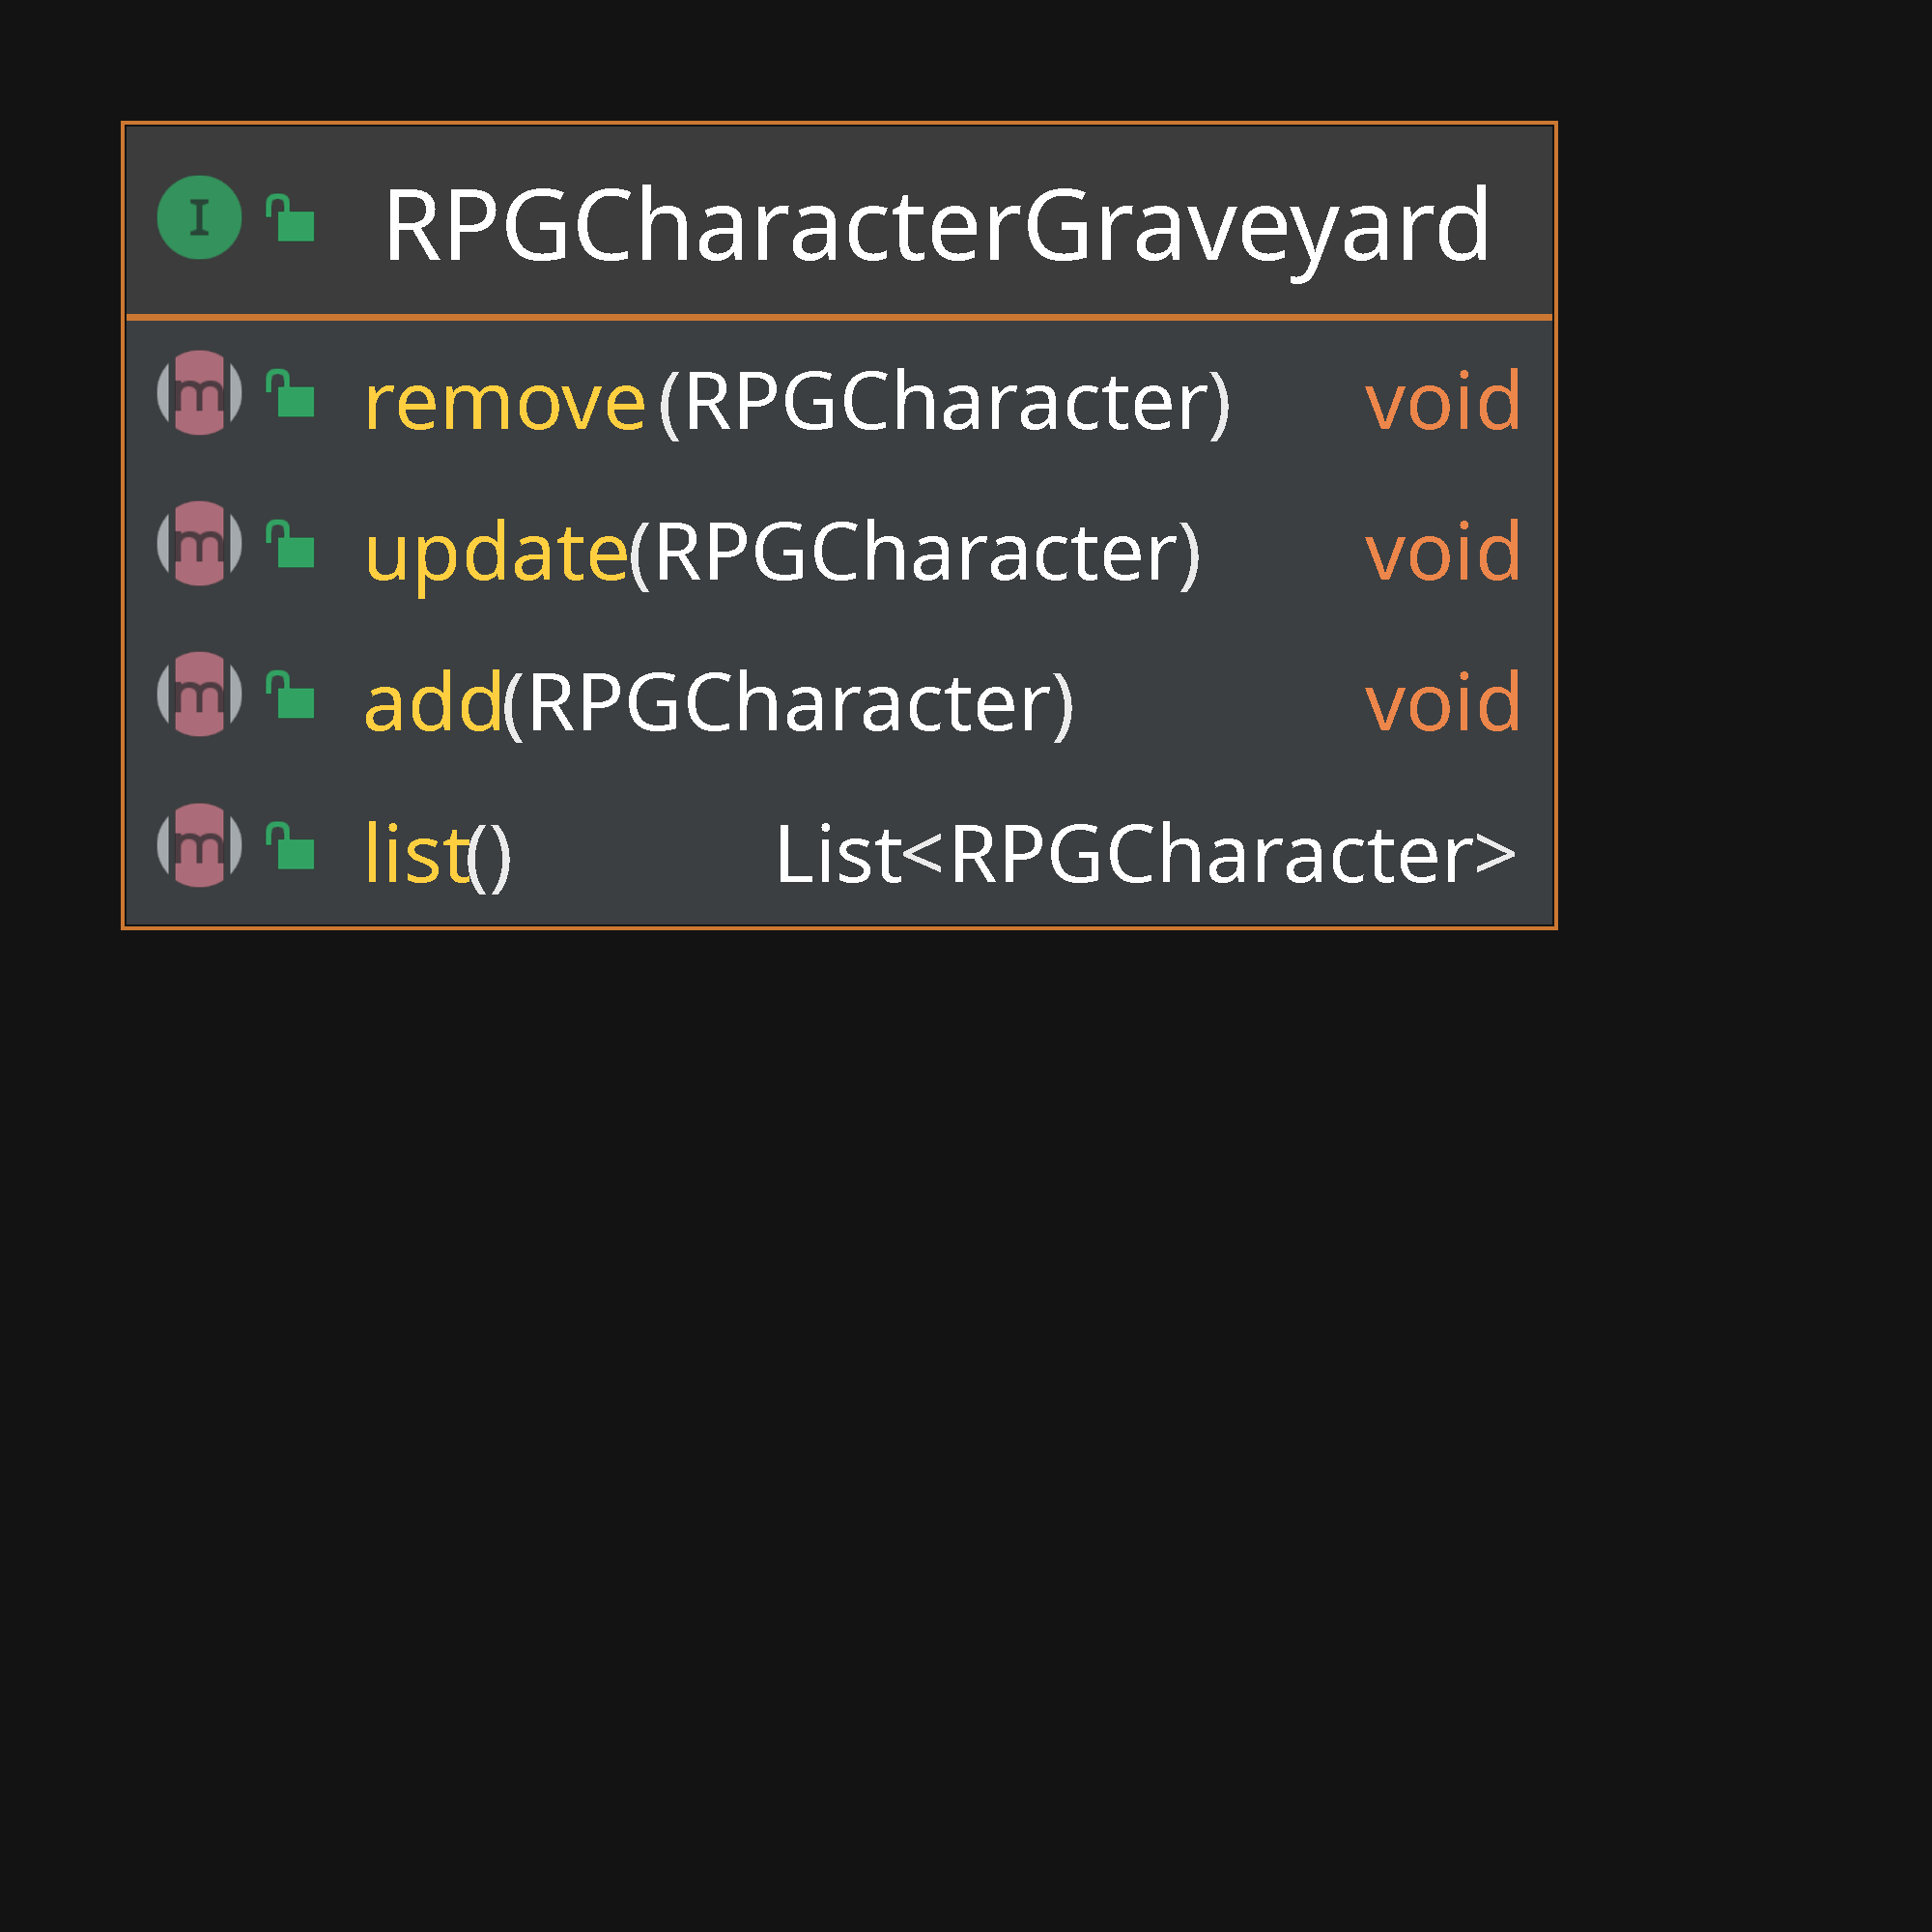
\includegraphics[width=0.4\textwidth]{Bilder/RPGCharacterGraveyard.pdf}
	\caption{UML des Repository Interface}
	\label{fig:Repository}
\end{figure}
Abbildung \ref{fig:Repository} zeigt das UML Klassendiagramm des \texttt{RPGCharacterGraveyard} Interfaces. Dieses Interface stellt die Schnittstelle / Implementierungsvorlage für die persistierung des Charakterfriedhofs dar. Da hier Daten persistiert und verwaltet werden bildet dies ein Repository.

\section{Aggregates}
\begin{figure}[H]
	\centering
	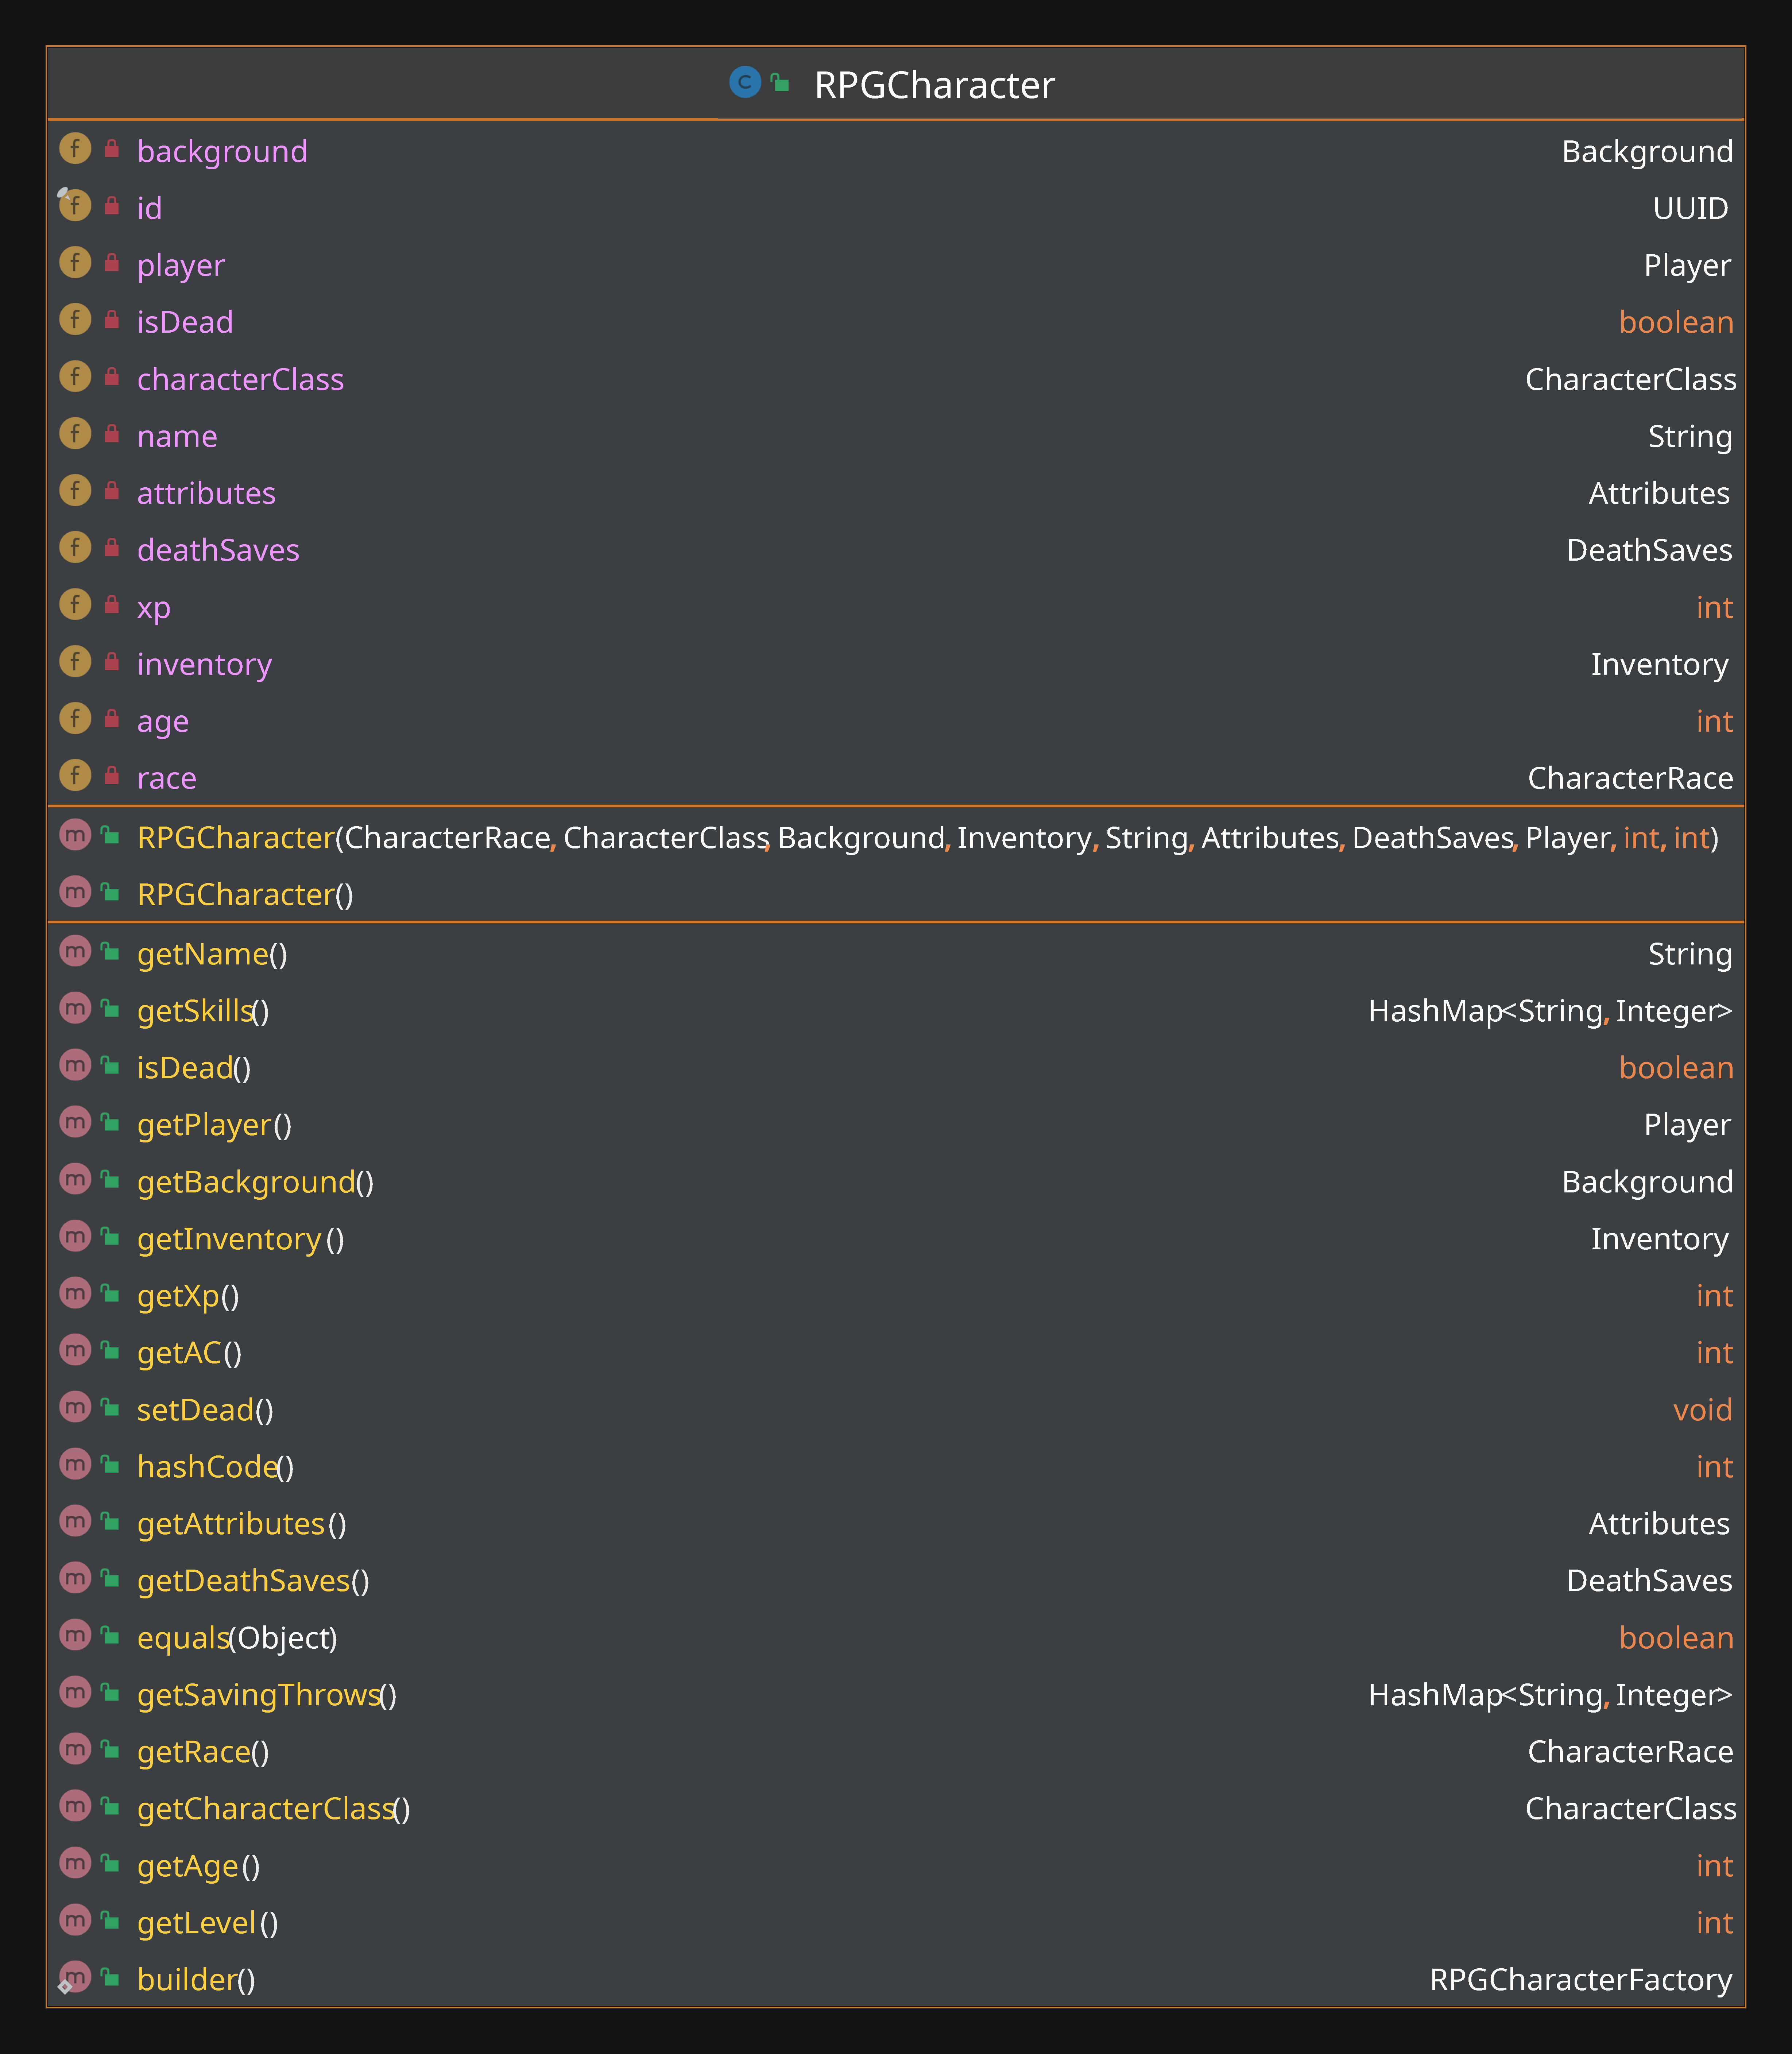
\includegraphics[width=0.4\textwidth]{Bilder/RPGCharacter.pdf}
	\caption{UML der RPGChracter Klasse}
	\label{fig:Aggregate}
\end{figure}
Abbildung \ref{fig:Aggregate} zeigt das UML Diagramm der Klasse \texttt{RPGCharacter}. Sie sammelt alle Eigenschaften eines Charakters und stellt sie in einem Zentralen Objekt zur Verfügung. Da auch diese Klasse unabhängig von ihrem Attributinhalt identifiziert werden muss, um z.b: Repositorys zu updaten, enthält sie eine ID. Da diese Klasse alle Eigenschaften eines Charakters sammelt und zentral zur Verfügung stellt, ist sie ein Aggragate.